\documentclass[french,a4paper]{article}
\setcounter{tocdepth}{4}
\setcounter{secnumdepth}{4}
\usepackage{float}
\usepackage{graphicx}
\usepackage{hyperref}
\usepackage{pdfpages}
\newcommand{\tabitem}{\textbullet~~}
\newcommand{\HRule}{\rule{\linewidth}{0.5mm}}
\usepackage{multirow}
\graphicspath{{img/}}
\title{PPII}
\usepackage[bottom=2.5cm,top=2.5cm,left=2.5cm,right=2.5cm]{geometry}
\author{Noé Steiner - Alexis Marcel - Lucas Laurent - Mathias Aurand-Augier}
\date{Janvier 2023}
\begin{document}

%\maketitle

\begin{titlepage}
    \begin{center}

    
\includegraphics[width=0.5\textwidth]{tele_univ.png}

    \textsc{\Large Rapport finale de Projet Pluridisciplinaire d'Informatique Intégrative}\\[1.5cm]

    \HRule \\[0.4cm]
    { \huge \bfseries Les jardins partagés\\[0.4cm] }

    \HRule \\[2cm]

    \begin{minipage}{0.4\textwidth}
      \begin{flushleft} \large
        Alexis MARCEL\\
        Lucas LAURENT\\
        Noé STEINER\\
        Mathias AURAND-AUGIER\\
      \end{flushleft}
    \end{minipage}
    \begin{minipage}{0.4\textwidth}
      \begin{flushright} \large
        \emph{Responsable du module :}\\
        Olivier FESTOR\\
        Anne-Claire HEURTEL\\
        Gerald OSTER\\
      \end{flushright}
    \end{minipage}

    \vfill

    {\large 6 Janvier 2023}

  \end{center}
\end{titlepage}
\newpage
\tableofcontents
\newpage
\section{Base de donnée}
\subsection{Conception}
\subsubsection{Que faut-il dans notre base ?}
\subsubsection{Schéma entité-association}
\subsubsection{Mise en 3ème forme normale}
\subsection{Implémentation}
\subsubsection{Connection à la base}
\subsubsection{SQL alchemy}

\newpage
\section{Implémentation Partie Web}
\subsection{Backend}
\subsubsection{}
\subsubsection{}
\subsubsection{}
\subsection{Frontend}
\subsubsection{}
\subsubsection{}
\subsubsection{}
\subsection{Test et performance}
\subsubsection{}
\subsubsection{}
\subsubsection{}

\newpage
\section{Algorithme}
\subsection{Principe de l'algorithme}
\subsection{Implémentation}
\subsection{Analyse en complexité}
\subsection{Test de validité de l'algorithme}
\subsection{Analyse de performance}

\newpage
\section{Gestion de projet}
\subsection{Équipe de projet}
Ce projet est un projet local réalisé en groupe de 4 personnes~:
\begin{itemize}
    \item Alexis MARCEL
    \item Lucas LAURENT
    \item Noé STEINER
    \item Mathias AURAND-AUGIER
\end{itemize}
Le comité de pilotage est constitué de~:
\begin{itemize}
    \item Anne-Claire HEURTEL
    \item Olivier FESTOR
    \item Gérald OSTER
\end{itemize}
Ces personnes constituent les parties prenantes de notre projet ainsi que les acteurs influents sur le livrables.
\begin{figure}[H]
    \centering
    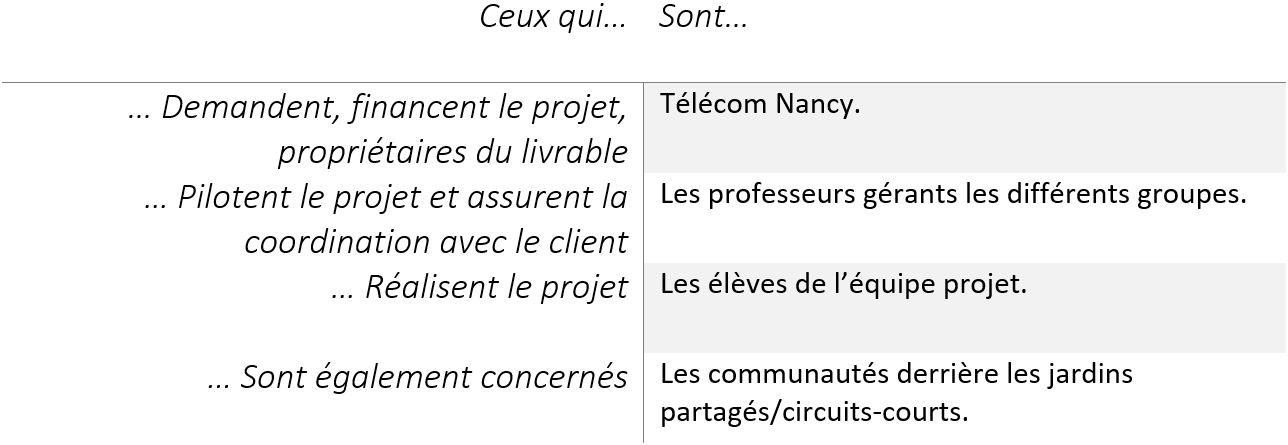
\includegraphics[width=0.75\textwidth]{img/parties_prenantes.png}
    \caption{Parties prenantes}
\end{figure} 
\subsection{Organisation au sein de l’équipe projet}
Nous avons réalisé plusieurs réunions, en présentiel dans les locaux de Télécom Nancy mais également sur en visio-conférence sur Discord. Ces réunions nous ont permis de mettre en commun nos avancés régulièrement, de partager nos connaissances sur des problématiques et de nous organiser de manière optimale.
Les comptes rendus des réunions réalisés sont présents dans l’\hyperlink{annexe1}{Annexe 1}.

De plus, dès le début de notre projet nous avons mis en place un projet Trello. Trello est une application permettant d’organiser facilement un projet en reposant sur une organisation en planches listant des cartes, chacune représentant des tâches. Ces tâches peuvent ensuite être déplacées permettant de découper notre projet en plusieurs jalons dynamiquement.
\begin{figure}[H]
    \centering
    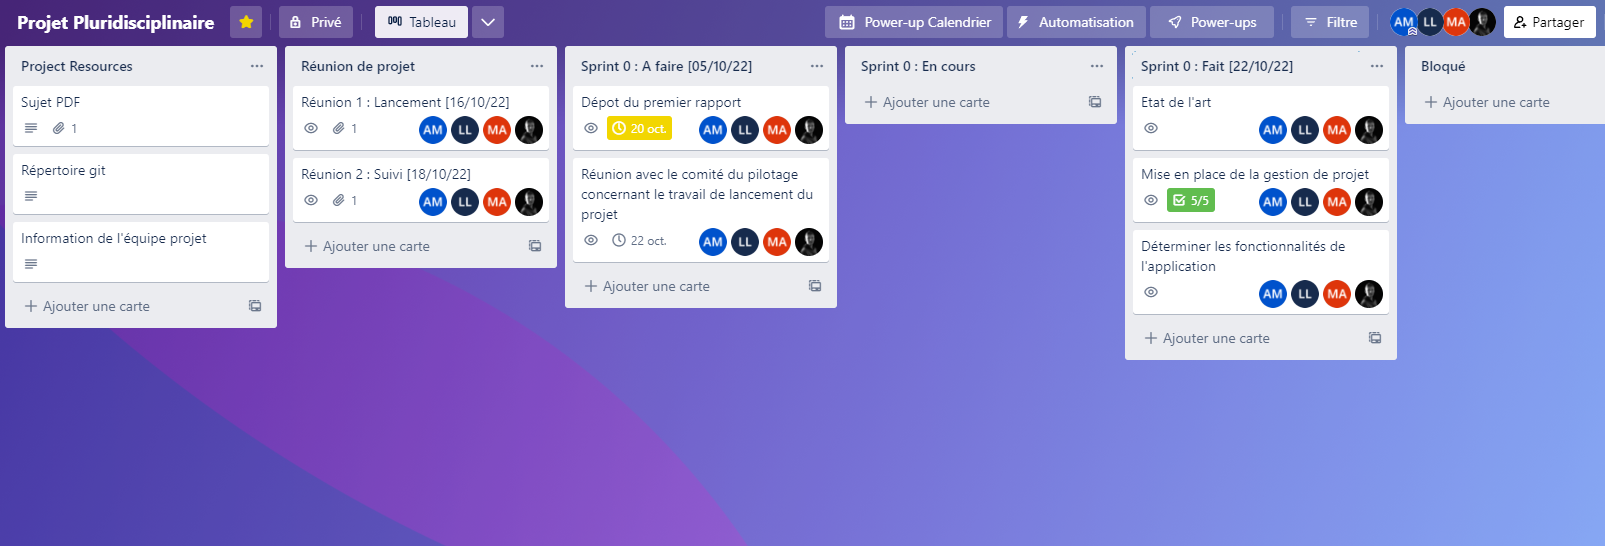
\includegraphics[width=0.75\textwidth]{img/trello.png}
    \caption{Organisation Trello}
\end{figure} 

Ensuite, nous avons utilisé GitLab pour gérer les différentes versions du développement de notre application, ainsi que les différentes branches nous permettant de travailler simultanément sans conflit.

Enfin, la rédaction des differents comptes rendu de réunion et des rapports ont été rédigé en \LaTeX.

\subsection{Objectifs SMART}
La méthode SMART que l'on rappelle ci-dessous nous a permis de définir nos différents objectifs :

\begin{figure}[H]
    \centering
    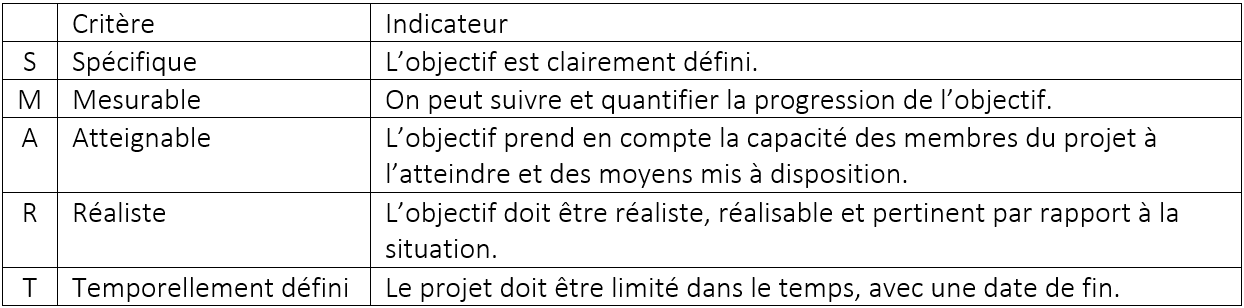
\includegraphics[width=1\textwidth]{img/SMART.png}
    \caption{Objectif SMART}
\end{figure}

\subsection{Matrice des objectifs}
Nous avons conçu, à l'aide de la méthode SMART, la matrice des objectifs suivante :

\begin{figure}[H]
    \centering
    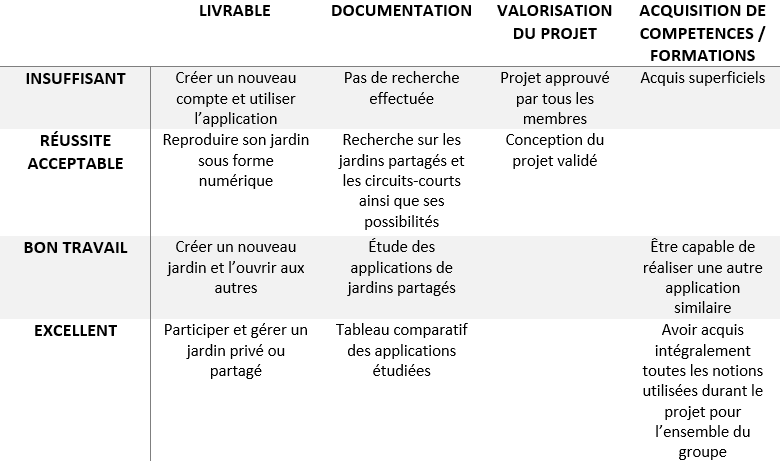
\includegraphics[width=1\textwidth]{img/matrice_des_objectifs.png}
    \caption{Matrice des objectifs}
\end{figure}

\subsection{Triangle qualité-cout-délai}
Afin d’établir des objectifs cohérents, et réalisables dans les délais, nous avons réalisé le triangle qualité-coût-délai. On remarque ainsi, les délais étant courts, que nous avons tout intérêt à ne pas se fixer des objectifs trop ambitieux sous peine de devoir renoncer à certaines fonctionnalités et de ne pas rendre le livrable annoncé initialement.

\begin{figure}[H]
    \centering
    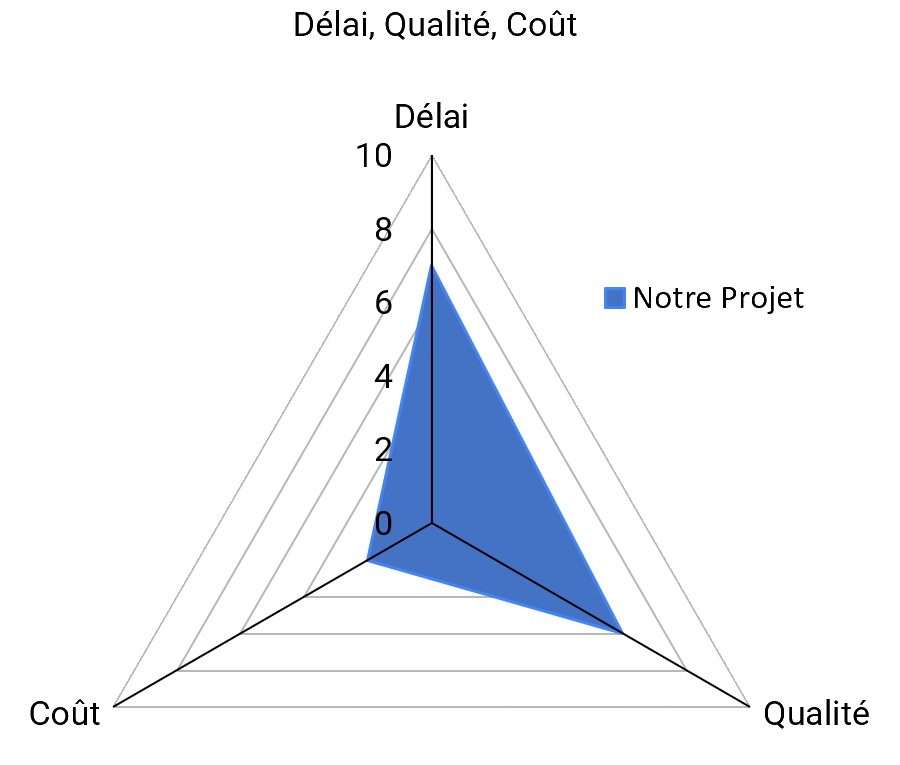
\includegraphics[width=0.5\textwidth]{img/triangle_QCD.png}
    \caption{Triangle DQC}
\end{figure}

\subsection{Matrice SWOT}
Afin d’avoir une vision plus globale de nos ressources et des facteurs interne et externe agissant sur le projet, nous avons ensuite réalisé la matrice SWOT (Strengths, Weaknesses, Opportunities, Threats) de notre projet.

\begin{figure}[H]
    \centering
    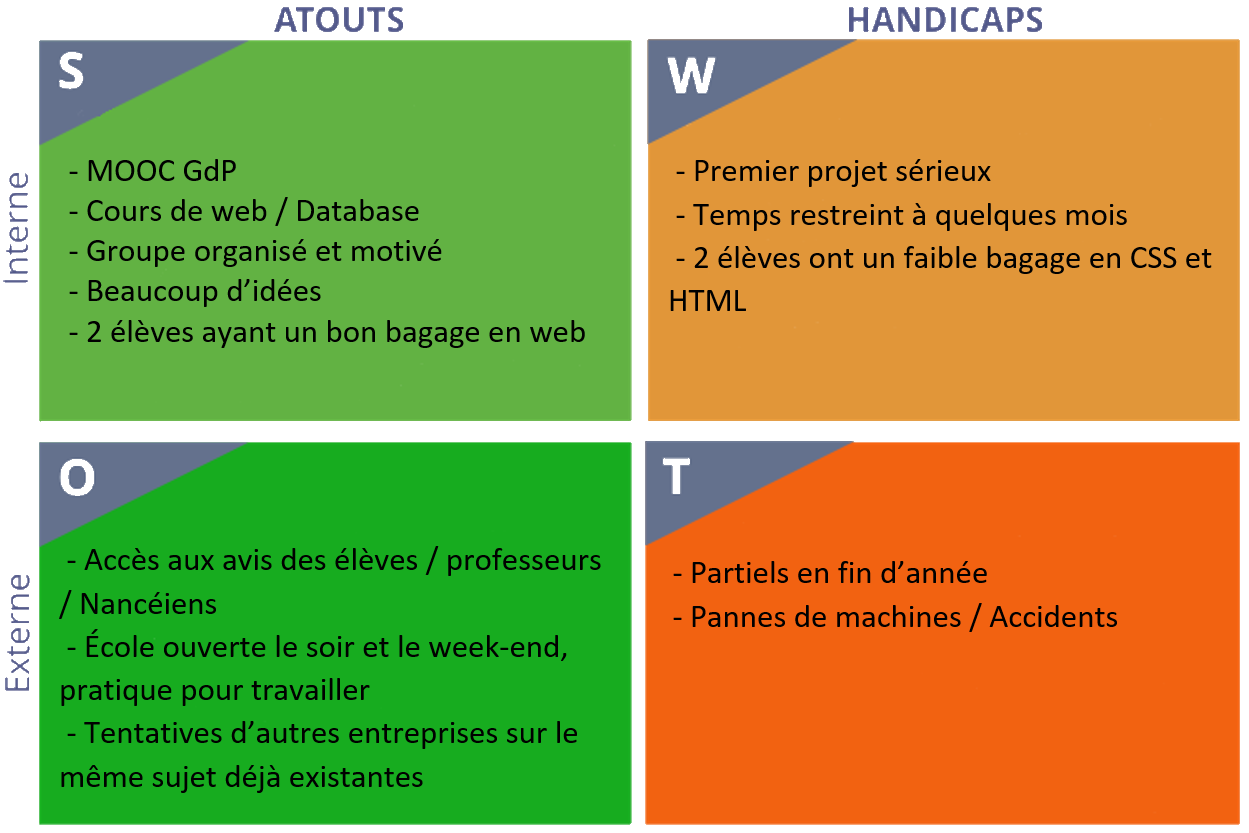
\includegraphics[width=0.75\textwidth]{img/SWOT.png}
    \caption{Matrice SWOT}
\end{figure} 

On peut ainsi remarquer que notre projet présente de nombreux points fort notamment grâce aux connaissances acquises lors des cours de Télécom Nancy mais également de part l’expérience forte de deux des membres de l’équipe projet qui ont déjà réalisé des applications similaires.  Cependant, plusieurs facteurs internes constituent nos faiblesses notamment les courts délais qui nous oblige à être concis et efficaces dans notre travail, ou encore le faible bagage informatique de deux des membres de l’équipe. Néanmoins, ces lacunes constituent pour eux l’opportunité d’apprendre, et de progresser avec l’aide des membres expérimentés de l’équipe.

De plus, nous devons anticiper les charges de travail dans le cadre de notre formation à Télécom Nancy qui s'avèrent être plus élevée en décembre lors des partiels de fin d'année. Nous allons donc devoir prendre cela en compte dans notre gestion des tâches. 

\subsection{Profil de projet}
Afin d’avoir une vision plus globale sur notre projet, nous avons également réalisé le profil du projet (le budget étant égal à 0, nous avons choisi de ne pas le représenter dans notre profil). On remarque que, du fait des nombreuses fonctionnalités que nous avons l’intention d’implémenter dans notre application, que notre projet est de taille moyenne mais de complexité élevée.

Cependant, les enjeux du projet ne sont pas très importants (en dehors de la note finale qui compte dans notre moyenne) car l'échec du projet n'engendra pas la chute d'une organisation et le budget est négligeable.

De plus, au vu de l’état de l’art établi, l’innovation du projet est importante puisque nous avons choisi de combiner différentes fonctionnalités existantes de plusieurs applications et d’en rajouter de nouvelles.

\begin{figure}[H]
    \centering
    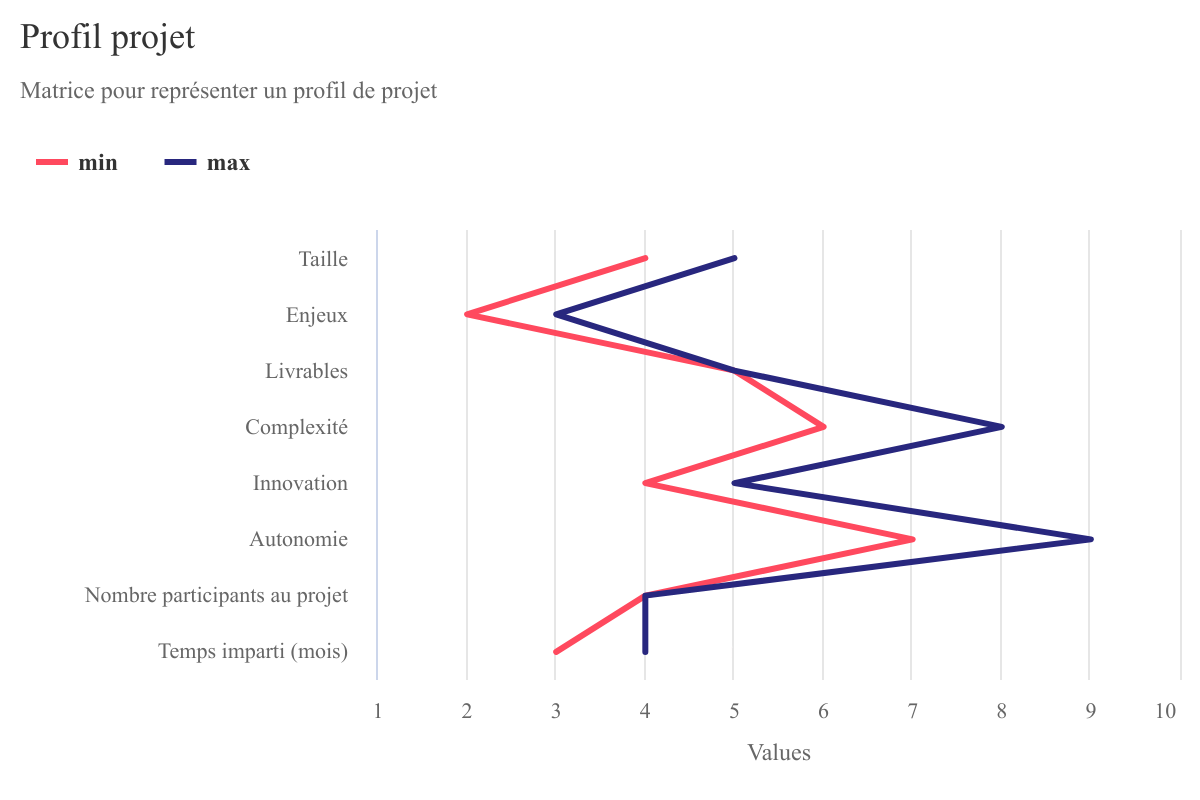
\includegraphics[width=0.75\textwidth]{img/profil_projet.png}
    \caption{Profil du projet}
\end{figure} 

\subsection{WBS~: comment concrétiser l’application}
Ceci étant fait, nous avons maintenant choisi de détailler les lots de travail à effectuer pour fabriquer notre application. Nous avons ainsi réalisé le WBS (Work Breakdown Structure) de notre application~: il apparait ainsi les grandes étapes de notre projet que sont~: definition du cadre de l’application, développement des fonctionnalités de l’application et écriture du rapport.
\begin{figure}[H]
    \centering
    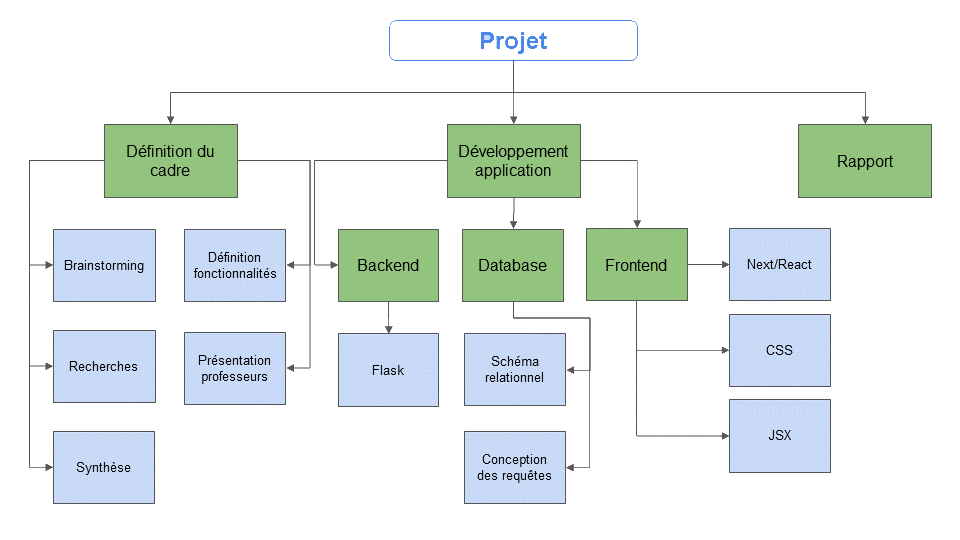
\includegraphics[width=0.75\textwidth]{img/WBS.png}
    \caption{WBS}
\end{figure} 

\subsection{Diagramme de Gantt~: planification}
Maintenant que nous avons un détail des lots de travail qui constitue notre application, il faut maintenant les mettre en relation pour créer un planning efficace où chaque tâche est effectuée dans l’ordre.
\begin{figure}[H]
    \centering
    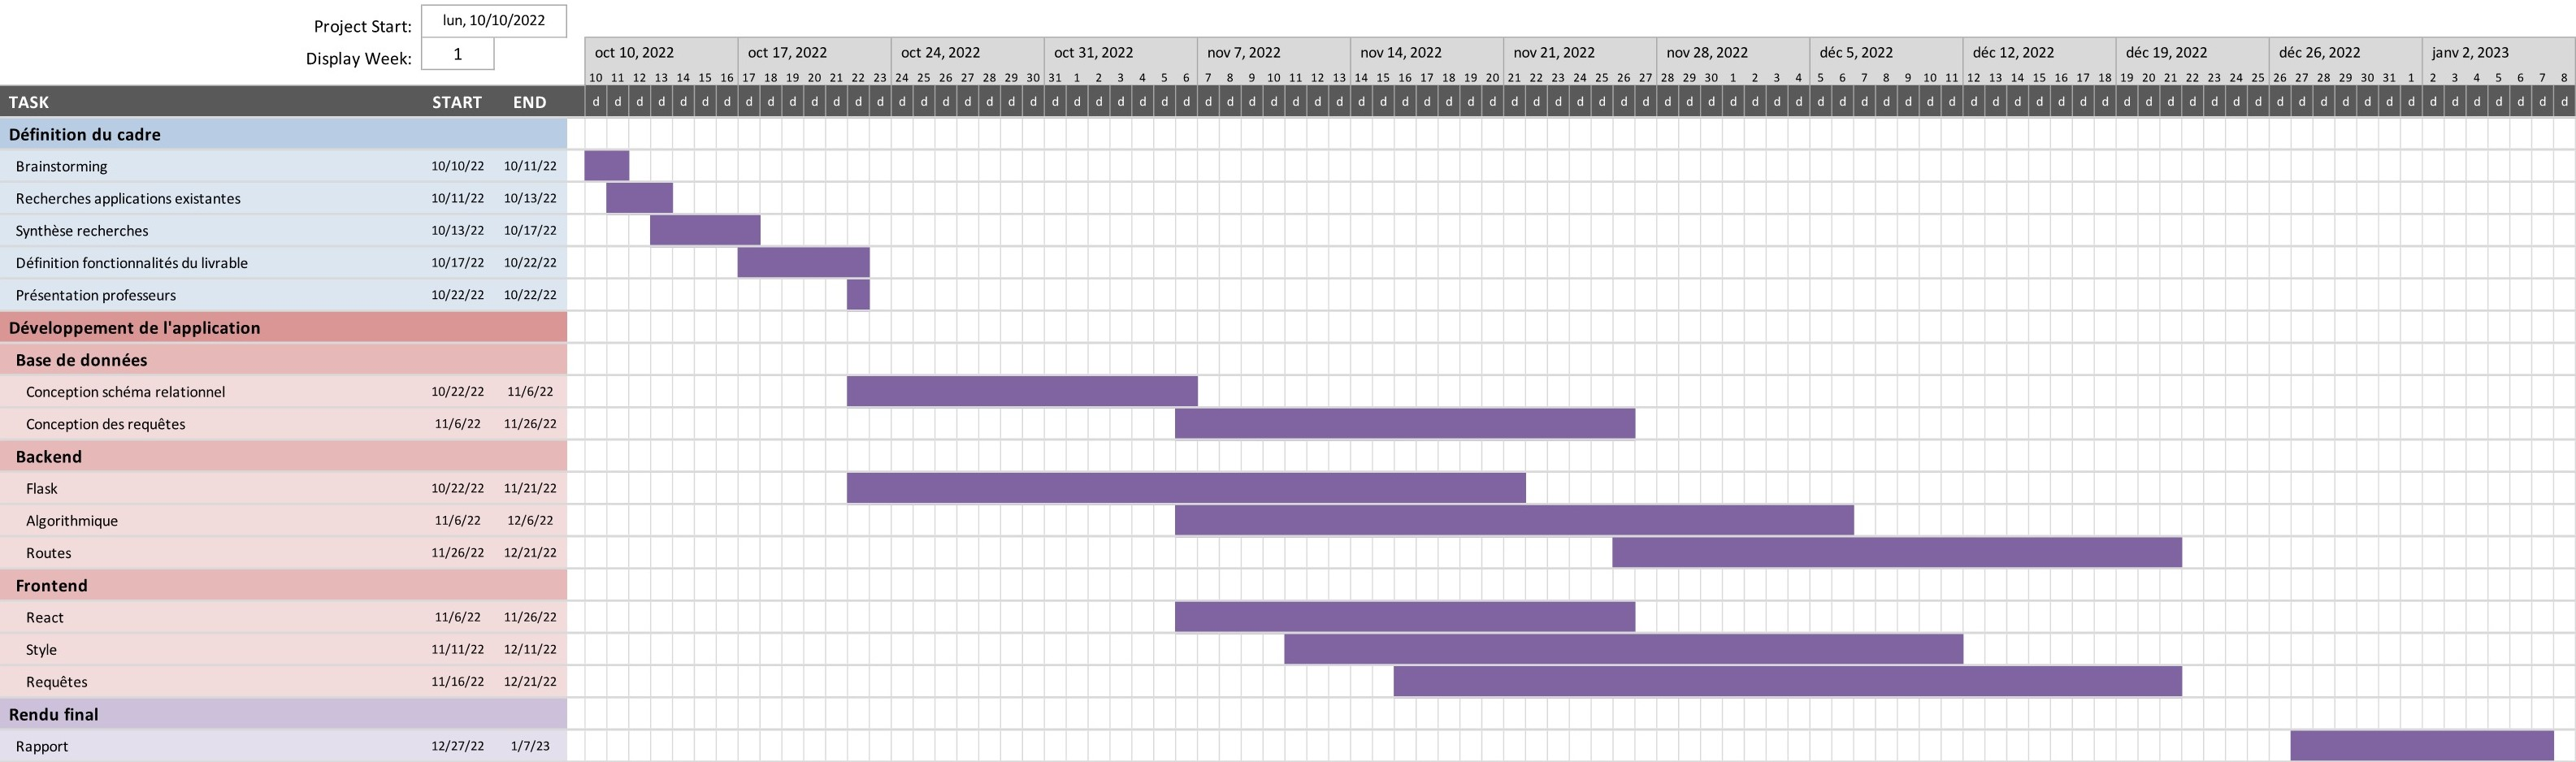
\includegraphics[width=1\textwidth]{img/gantt.png}
    \caption{Diagramme de GANTT}
\end{figure} 
Ce diagramme est une première version générale des tâches à effectuer, il sera modifié et détaillé davantage une fois la conception et les maquettes du projet réalisé.

\subsection{Matrice RACI}
Maintenant que toutes les étapes sont planifiées, nous devons répartir le travail entre les membres de l’équipe. On utilise ainsi une matrice RACI synthétisant les rôles de chacun.

\begin{figure}[H]
    \centering
    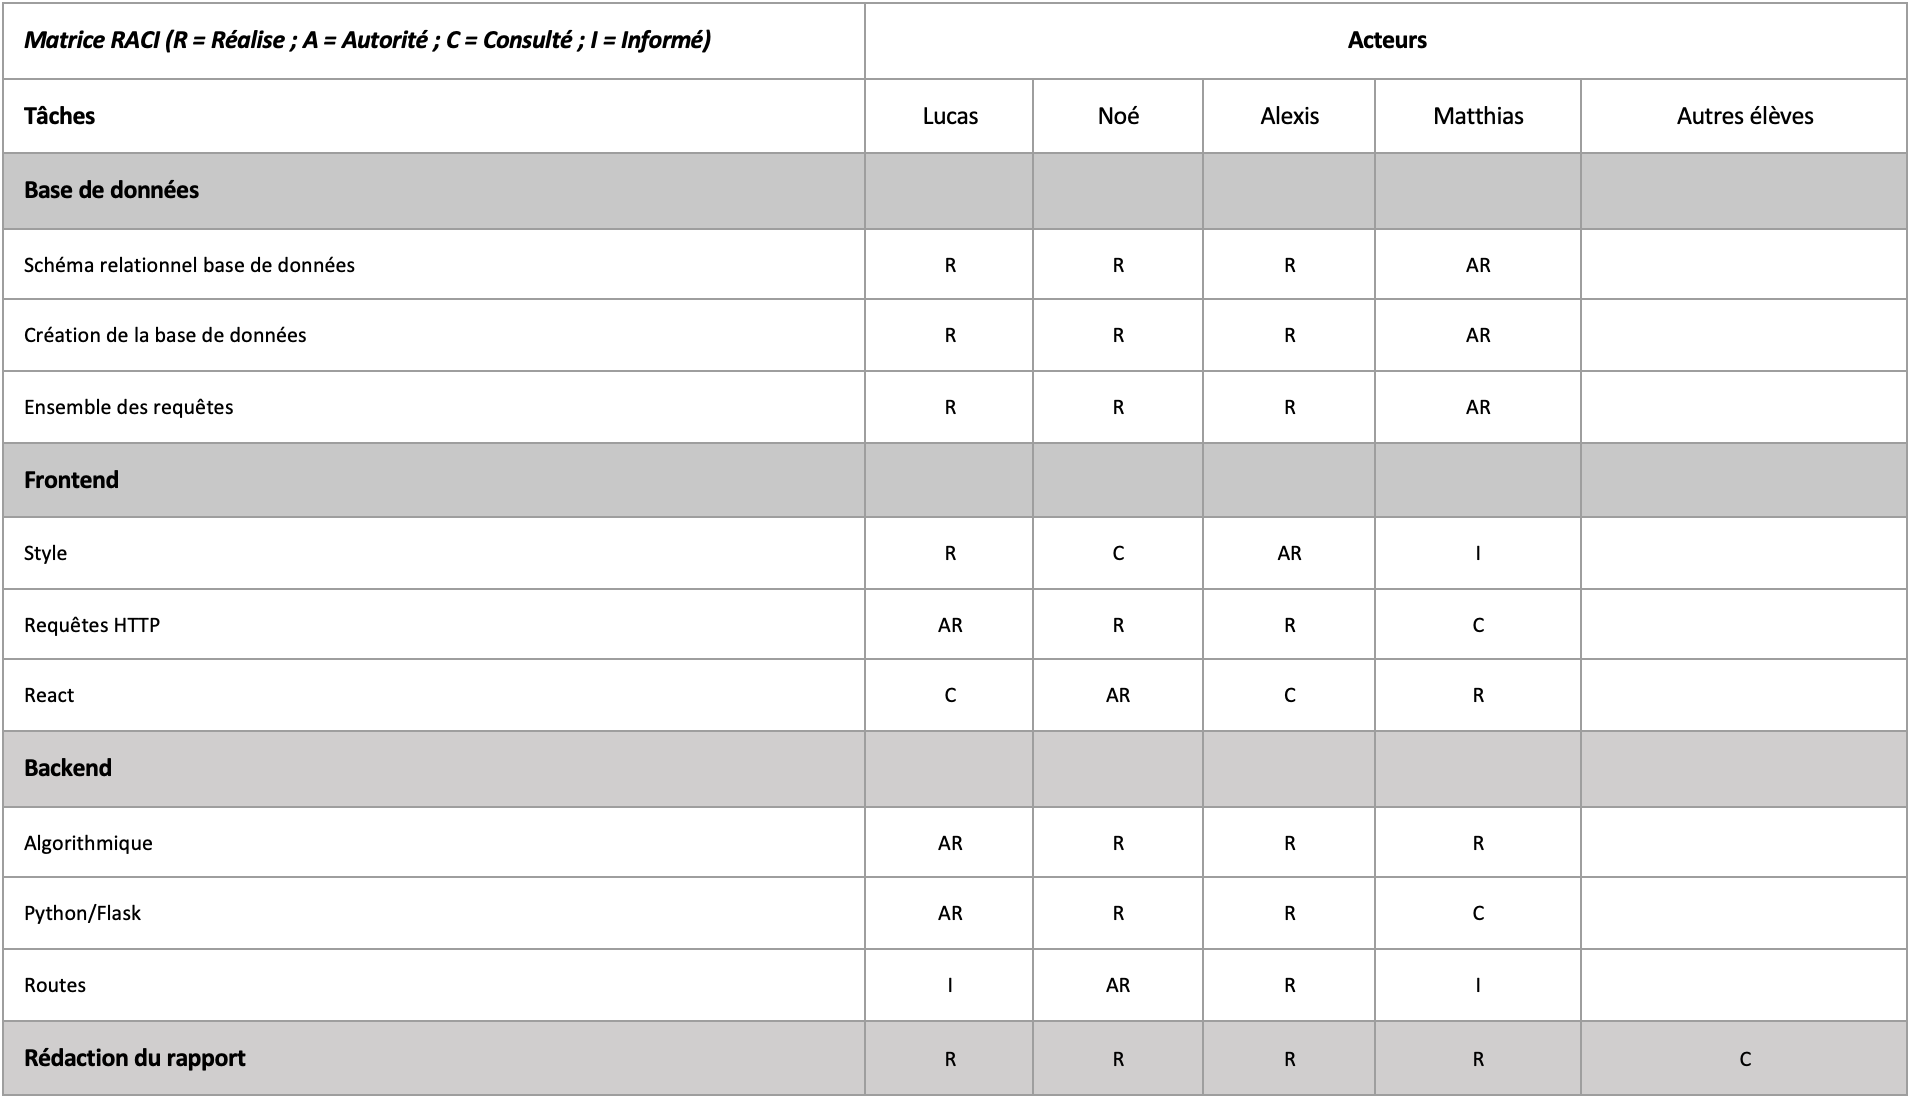
\includegraphics[width=1\textwidth]{img/RACI.png}
    \caption{Matrice RACI}
\end{figure} 

\section{Conclusion}

\section{Annexe}
\subsection[Annexe1]{Annexe 1\hypertarget{annexe1}{}}

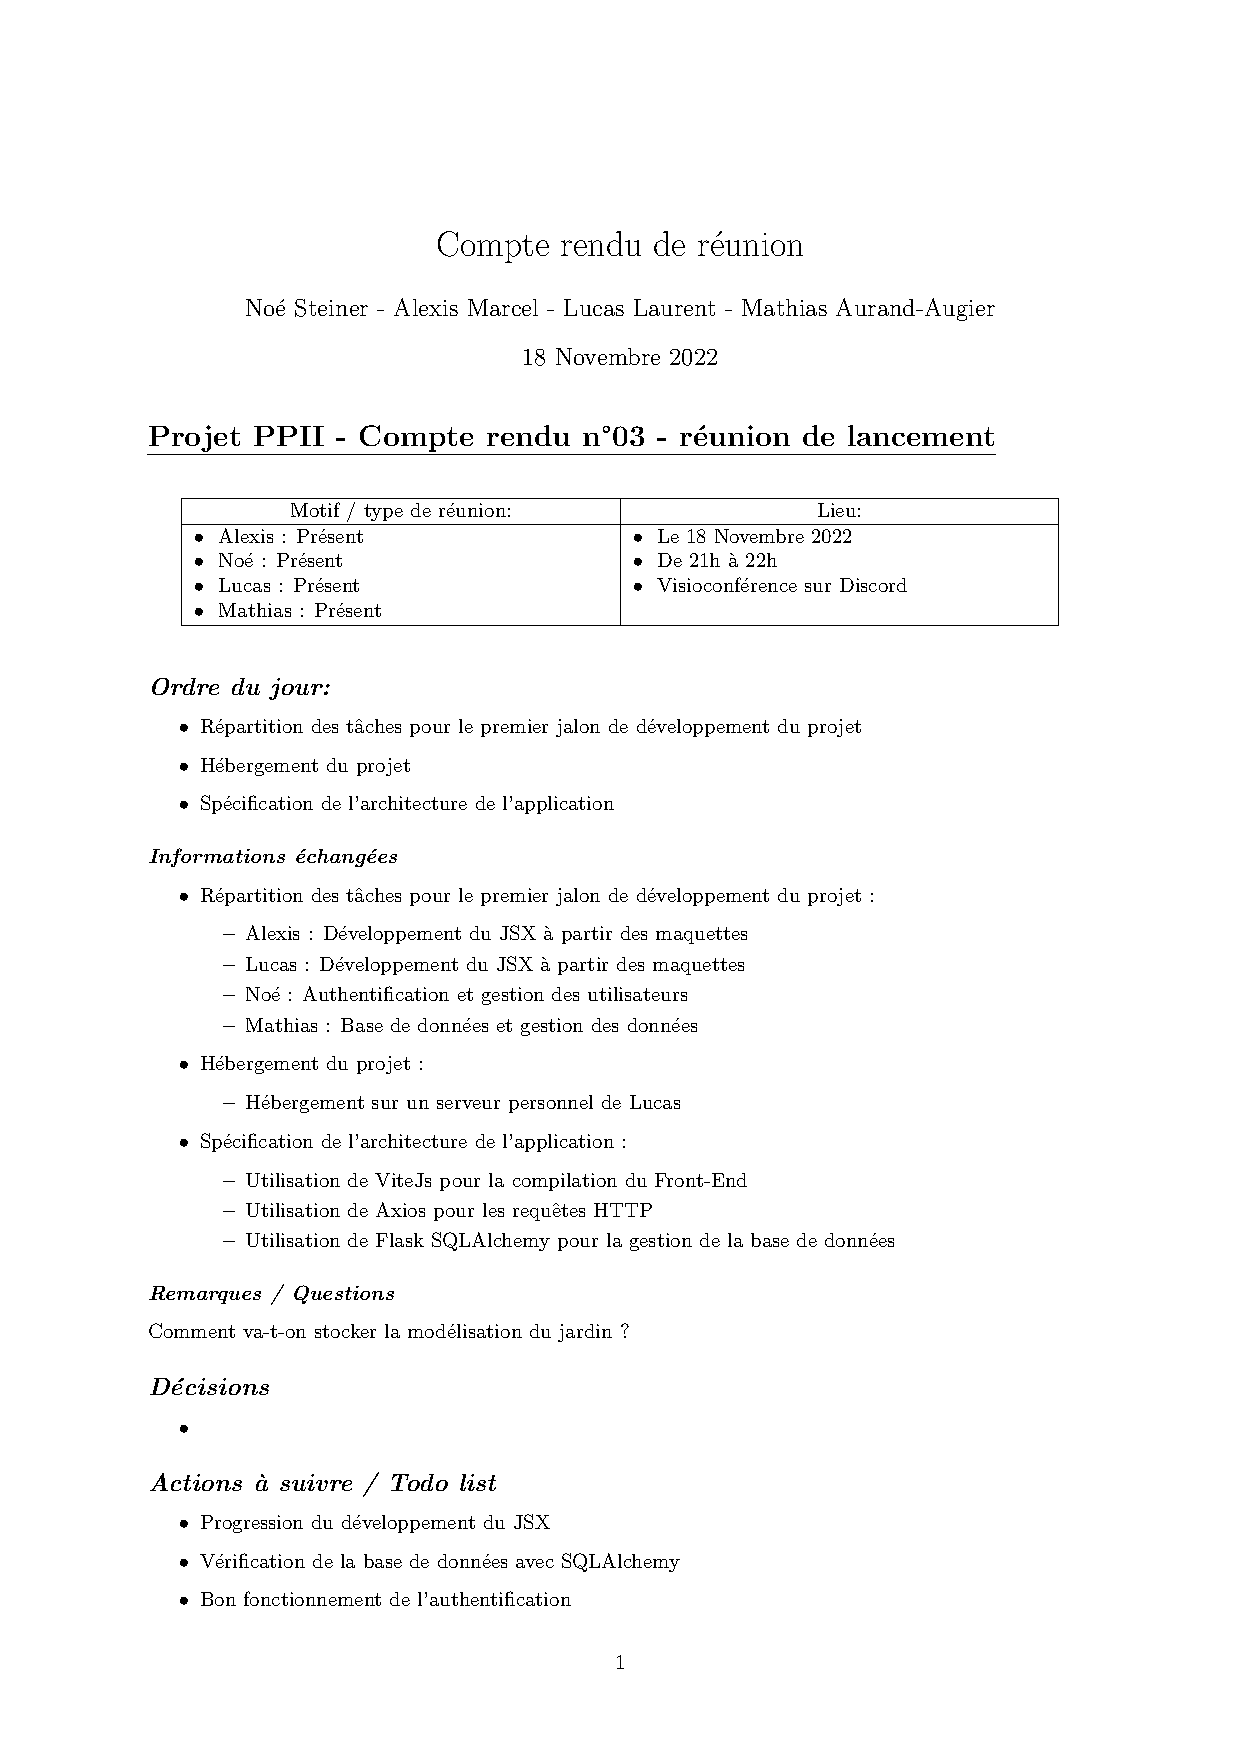
\includepdf[pages=1]{../../cr_reu/novembre/cr_18_novembre.pdf}
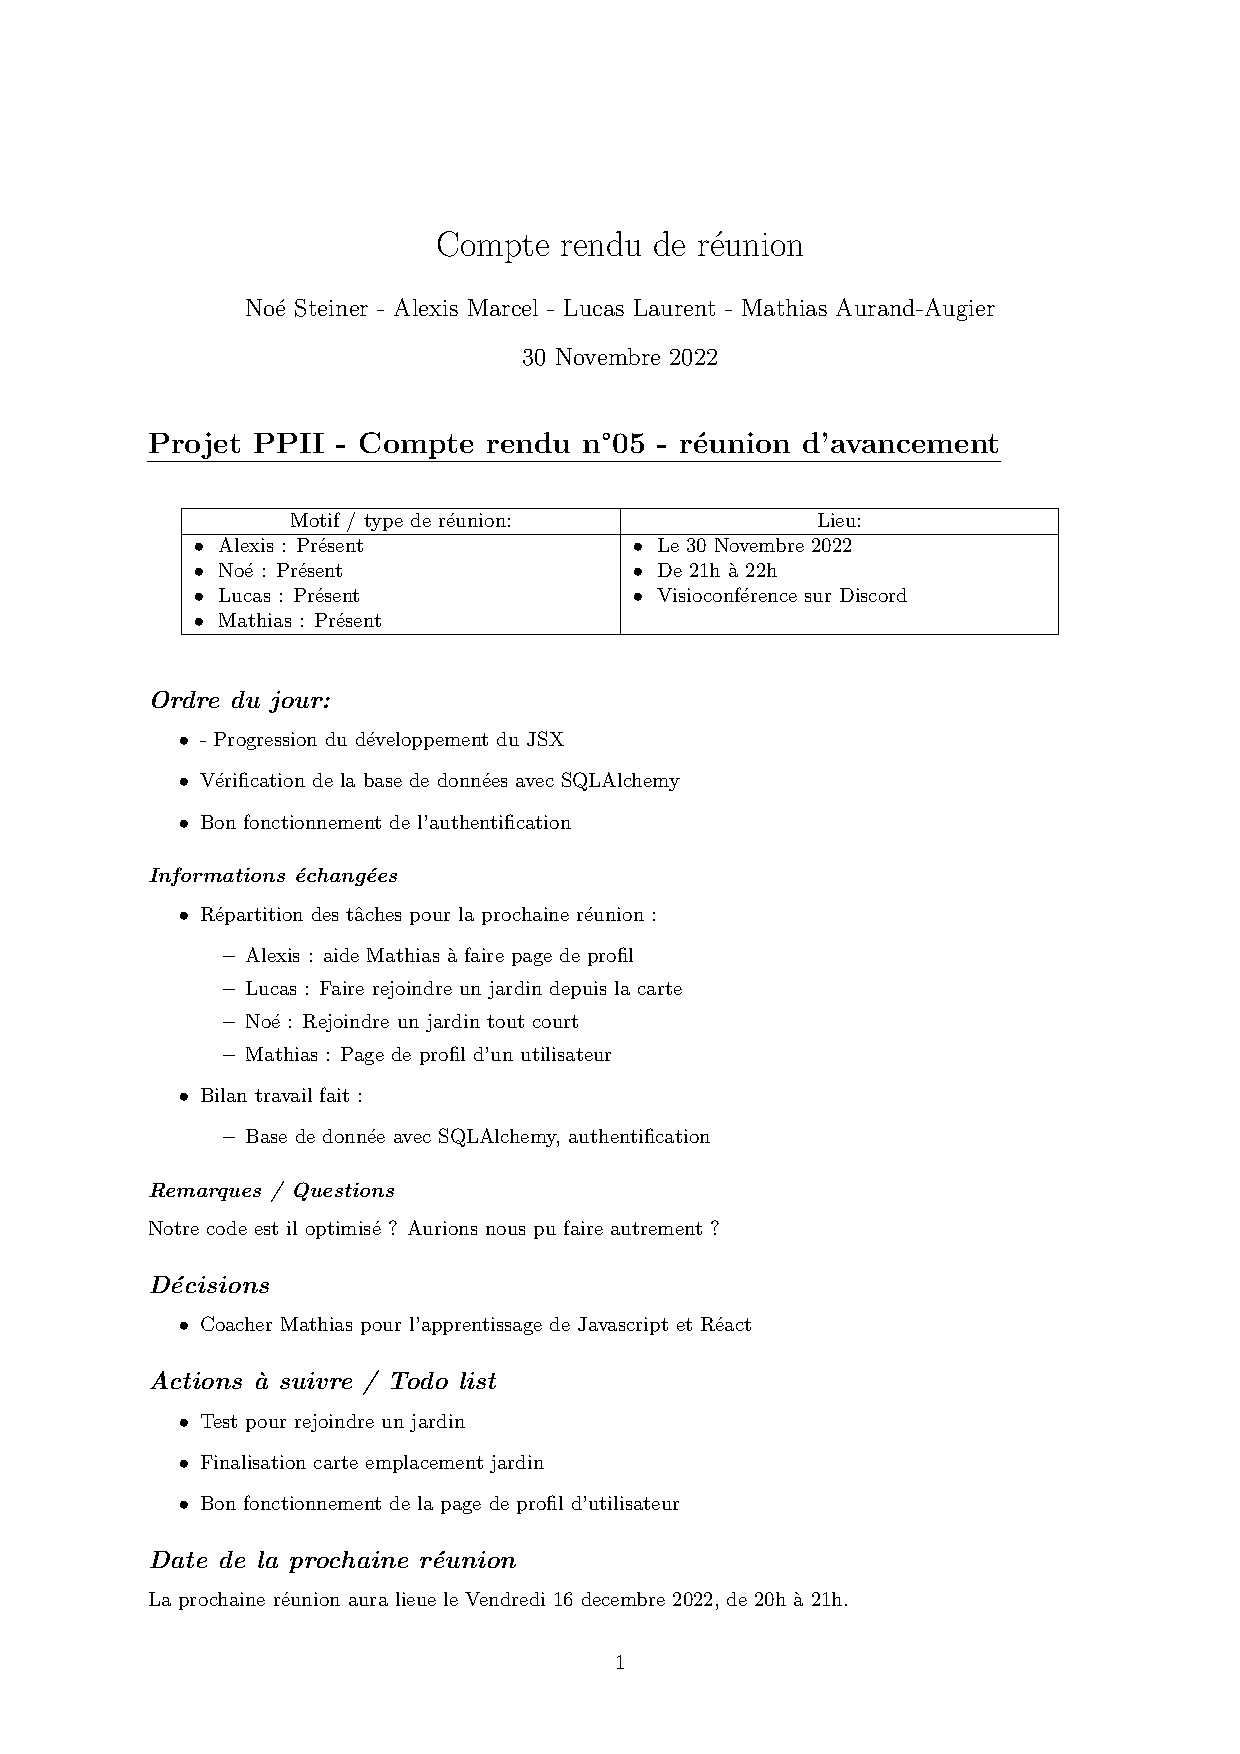
\includepdf[pages=1]{../../cr_reu/novembre/cr_30_novembre.pdf}
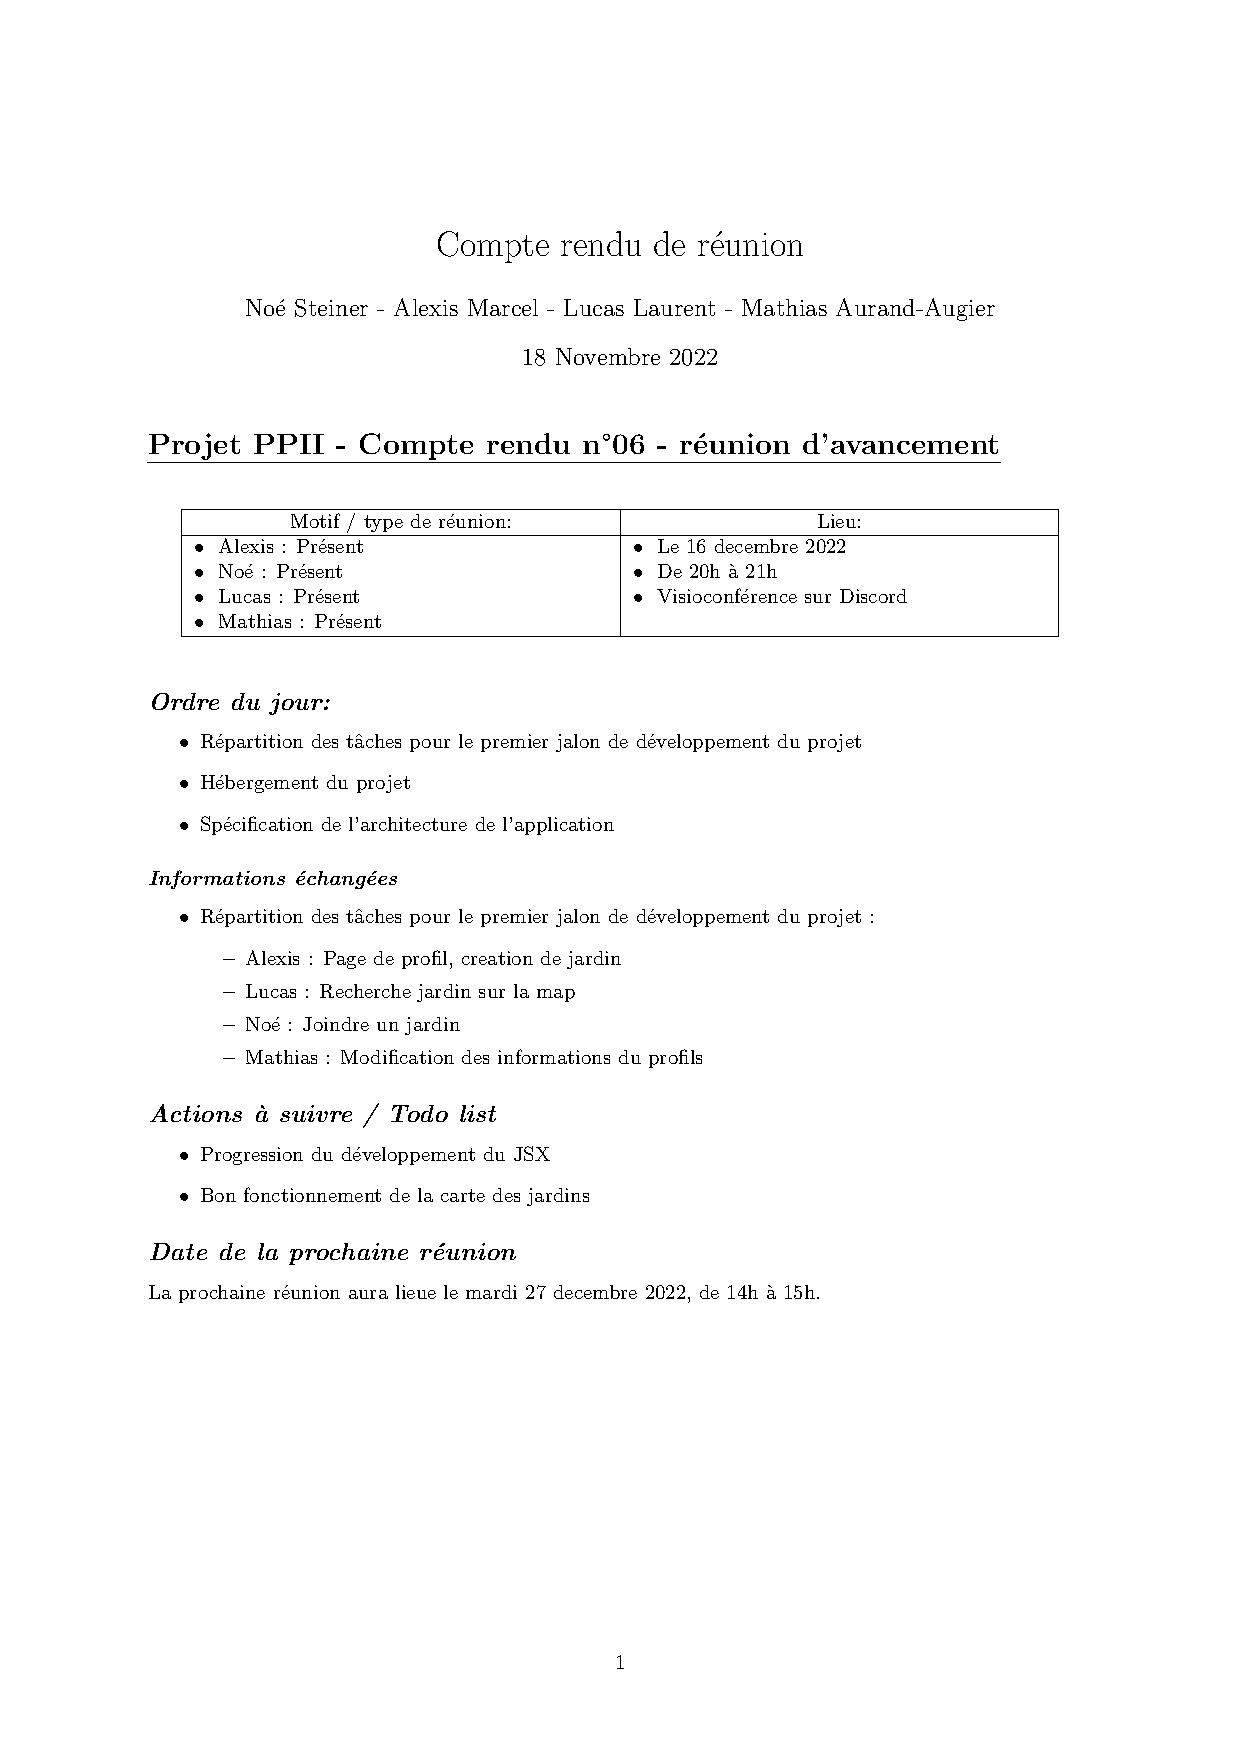
\includepdf[pages=1]{../../cr_reu/decembre/cr_16_decembre.pdf}
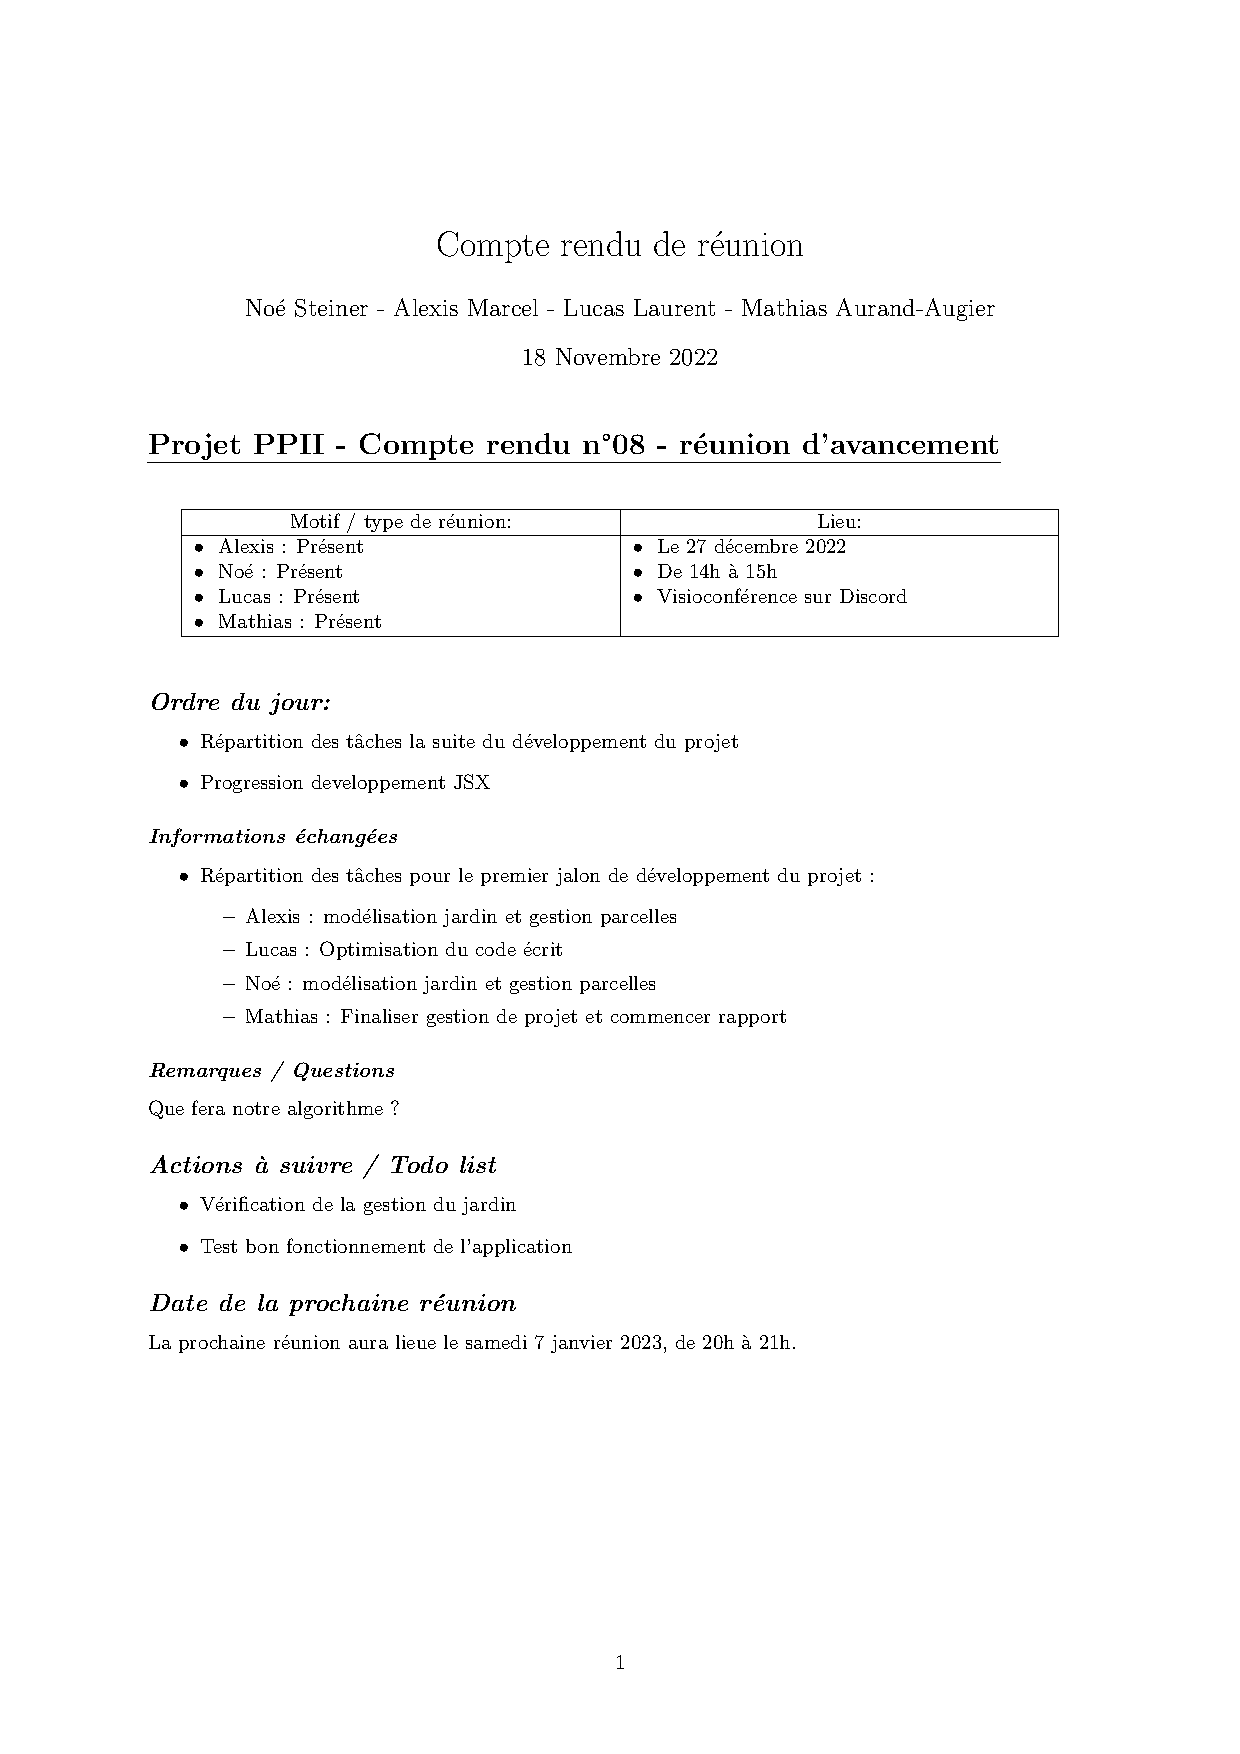
\includepdf[pages=1]{../../cr_reu/decembre/cr_27_decembre.pdf}
\end{document}